\documentclass[12pt,letterpaper]{exam}
\usepackage[lmargin=1in,rmargin=1in,tmargin=1in,bmargin=1in]{geometry}
\usepackage{../style/exams}

% -------------------
% Course & Exam Information
% -------------------
\newcommand{\course}{MAT 107: Exam 2}
\newcommand{\term}{Winter -- 2022}
\newcommand{\examdate}{01/16/2023}
\newcommand{\timelimit}{Time Limit: `$\infty$'}

\setbool{hideans}{false} % Student: True; Instructor: False

% i, j, k
\usepackage{bm}
\newcommand{\uveci}{{\bm{\hat{\textnormal{\bfseries\i}}}}}
\newcommand{\uvecj}{{\bm{\hat{\textnormal{\bfseries j}}}}}
\newcommand{\uveck}{{\bm{\hat{\textnormal{\bfseries k}}}}}

% -------------------
% Content
% -------------------
\begin{document}

\examtitle
\instructions{Write your name on the appropriate line on the exam cover sheet. This exam contains \numpages\ pages (including this cover page) and \numquestions\ questions. Check that you have every page of the exam. Answer the questions in the spaces provided on the question sheets. Be sure to answer every part of each question and show all your work. If you run out of room for an answer, continue on the back of the page --- being sure to indicate the problem number.} 
\scores
\bottomline
\newpage

% ---------
% Questions
% ---------
\begin{questions}

% Question 1
\newpage
\question[10] Define the following vectors:
	\[
	\begin{tikzpicture}
	\node at (-1.7,-0.25) {$\vec{u}$};
	\draw[line width=0.03cm,->] (0,0) -- (-3,-1);
	
	\tikzset{shift={(1,0)}}
	
	\node at (0.45,-0.3) {$\vec{v}$};
	\draw[line width=0.03cm,->] (0,0) -- (0.4,-1);
	
	\tikzset{shift={(2,0)}}
	
	\node at (1.5,0.3) {$\vec{w}$};
	\draw[line width=0.03cm,->] (0,0) -- (3,0);
	\end{tikzpicture}
	\]
As accurately as possible, sketch the following:
	\begin{enumerate}[(a)]
	\item $\vec{u} + \vec{w}$
	\item $\vec{v} - \vec{u}$
	\item $-\frac{1}{2}\, \vec{w}$
	\item $\vec{u} + 2 \vec{v}$
	\end{enumerate} \pspace

\sol 
\begin{enumerate}[(a)]
\item 
	\[
	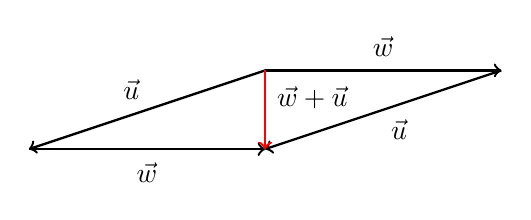
\begin{tikzpicture}
	\node at (1.7,-0.75) {$\vec{u}$};
	\node at (1.5,0.3) {$\vec{w}$};
	\draw[line width=0.03cm,->] (0,0) -- (-3,-1);
	\draw[line width=0.03cm,->] (-3,-1) -- (0,-1);
	
	\node at (-1.5,-1.3) {$\vec{w}$};
	\node at (-1.7,-0.25) {$\vec{u}$};
	\draw[line width=0.03cm,->] (0,0) -- (3,0);
	\draw[line width=0.03cm,->] (3,0) -- (0,-1);
	
	\node at (0.6,-0.35) {$\vec{w} + \vec{u}$};
	\draw[line width=0.03cm,->,red] (0,0) -- (0,-1);
	\end{tikzpicture}
	\]

\item 
	\[
	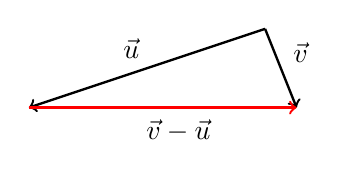
\begin{tikzpicture}
	\node at (-1.7,-0.25) {$\vec{u}$};
	\draw[line width=0.03cm,->] (0,0) -- (-3,-1);
	
	\node at (0.45,-0.3) {$\vec{v}$};
	\draw[line width=0.03cm,->] (0,0) -- (0.4,-1);
	
	\node at (-1.1,-1.3) {$\vec{v} - \vec{u}$};
	\draw[line width=0.03cm,->,red] (-3,-1) -- (0.4,-1);
	\end{tikzpicture}
	\]

\item 
	\[
	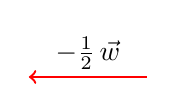
\begin{tikzpicture}
	\node at (0.75,0.3) {$-\frac{1}{2}\, \vec{w}$};
	\draw[line width=0.03cm,->,red] (1.5,0) -- (0,0);
	\end{tikzpicture}
	\]

\item 
	\[
	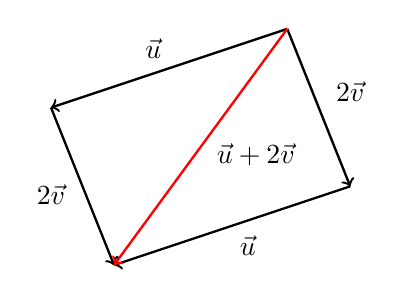
\begin{tikzpicture}
	\node at (-1.7,-0.25) {$\vec{u}$};
	\node at (-3,-2.1) {$2\vec{v}$};
	\draw[line width=0.03cm,->] (0,0) -- (-3,-1);
	\draw[line width=0.03cm,->] (-3,-1) -- (-2.2,-3);

	\node at (0.8,-0.8) {$2\vec{v}$};
	\node at (-0.5,-2.75) {$\vec{u}$};
	\draw[line width=0.03cm,->] (0,0) -- (0.8,-2);
	\draw[line width=0.03cm,->] (0.8,-2) -- (-2.2,-3);
	
	\node at (-0.4,-1.6) {$\vec{u} + 2\vec{v}$};
	\draw[line width=0.03cm,->,red] (0,0) -- (-2.2,-3);
	\end{tikzpicture}
	\]
\end{enumerate}



% Question 2
\newpage
\question[10] Let $\vec{u}= \langle 2, -1, 0 \rangle$ and $\vec{v}= \uveci + 4 \uvecj - \uveck$. Find the following:
	\begin{enumerate}[(a)]
	\item $-3 \vec{u}$
	\item $\vec{v} - \vec{u}$
	\item $3 \vec{u} + 2 \vec{v}$
	\item $\vec{u} \cdot \vec{v}$
	\item The angle between $\vec{u}$ and $\vec{v}$. 
	\end{enumerate} \pspace

\sol Note that $\vec{v}= \uveci + 4 \uvecj - \uveck= \langle 1, 4, -1 \rangle$. 
\begin{enumerate}[(a)]
\item 
	\[
	-3 \vec{u}= -3 \langle 2, -1, 0 \rangle= \langle -3(2), -3(-1), -3(0) \rangle= \langle -6, 3, 0 \rangle 
	\] \pspace

\item 
	\[
	\vec{v} - \vec{u}= \langle 1, 4, -1 \rangle - \langle 2, -1, 0 \rangle= \langle 1 - 2, 4 - (-1), -1 - 0 \rangle= \langle -1, 5, -1 \rangle 
	\] \pspace

\item 
	\[
	\begin{aligned}
	3 \vec{u} + 2 \vec{v}&= 3 \langle 2, -1, 0 \rangle + 2 \langle 1, 4, -1 \rangle \\[0.3cm]
	&= \langle 6, -3, 0 \rangle + \langle 2, 8, -2 \rangle \\[0.3cm]
	&= \langle 6 + 2, -3 + 8, 0 + (-2) \rangle \\[0.3cm]
	&= \langle 8, 5, -2 \rangle 
	\end{aligned}
	\] \pspace

\item 
	\[
	\vec{u} \cdot \vec{v}= \langle 2, -1, 0 \rangle \cdot \langle 1, 4, -1 \rangle= 2(1) + (-1)4 + 0(-1)= 2 - 4 + 0= -2
	\] \pspace

\item Recall that $\mathbf{u} \cdot \mathbf{v}= \| \mathbf{u} \| \| \mathbf{v} \| \cos \theta$. We have\dots
	\[
	\begin{aligned}
	\| \mathbf{u} \|&= \sqrt{2^2 + (-1)^2 + 0^2}= \sqrt{4 + 1 + 0}= \sqrt{5} \\[0.3cm]
	\| \mathbf{v} \|&= \sqrt{1^2 + 4^2 + (-1)^2}= \sqrt{1 + 16 + 1}= \sqrt{18}
	\end{aligned}
	\]
We know from (d) that $\mathbf{u} \cdot \mathbf{v}= -2$. Therefore, we have\dots
	\[
	\begin{aligned}
	\mathbf{u} \cdot \mathbf{v}&= \| \mathbf{u} \| \| \mathbf{v} \| \cos \theta \\[0.1cm]
	-2&= \sqrt{5} \cdot \sqrt{18} \cos \theta \\[0.1cm]
	-2&= 9.4868329805 \cos \theta \\[0.1cm]
	\cos \theta&= -0.21081851 \\[0.1cm]
	\theta&= \cos^{-1}(-0.21081851) \\[0.1cm]
	\theta&\approx 102.17^\circ
	\end{aligned}
	\]
\end{enumerate}



% Question 3
\newpage
\question[10] Suppose you are a sprite in a 2D video game. Currently, you are at $\vec{p}= \langle 2.4, 3.7 \rangle$. You are moving in the direction given by $\langle -2, 1 \rangle$ at speed 1.6. Find your position one game `tick' from now. \pspace

\sol We have\dots
	\[
	\| \langle -2, 1 \rangle \|= \sqrt{(-2)^2 + 1^2}= \sqrt{4 + 1}= \sqrt{5}
	\]
The velocity vector is then\dots
	\[
	\vec{v}= 1.6 \cdot \dfrac{\langle -2, 1 \rangle}{\sqrt{5}}= 0.7155 \langle -2, 1 \rangle= \langle -1.431, 0.7155 \rangle 
	\]
Then we have\dots
	\[
	\begin{aligned}
	\vec{p}_N&= \vec{p}_0 + \Delta \vec{p} \\[0.3cm]
	&= \vec{p}_0 + t \vec{v} \\[0.3cm]
	&= \langle 2.4, 3.7 \rangle + 1 \cdot \langle -1.431, 0.7155 \rangle \\[0.3cm]
	&= \langle 0.969, 4.4155 \rangle 
	\end{aligned}
	\]



% Question 4
\newpage
\question[10] Define the following:
	\[
	A= 
	\begin{pmatrix}
	1 & 0 & -2 \\
	0 & 4 & 1 \\
	-6 & 1 & 3
	\end{pmatrix},
	\qquad
	B= 
	\begin{pmatrix}
	0 & -1 & 5 \\
	3 & 2 & 1 \\
	-2 & 1 & 0 
	\end{pmatrix},
	\qquad
	C= 
	\begin{pmatrix}
	1 & 4 & 0 \\
	2 & -1 & 5 
	\end{pmatrix}
	\]
Find the following:
	\begin{enumerate}[(a)]
	\item $4C$
	\item $A - B$
	\item $CA$
	\end{enumerate} \pspace

\sol 
\begin{enumerate}[(a)]
\item 
	\[
	4C=
	4 
	\begin{pmatrix}
	1 & 4 & 0 \\
	2 & -1 & 5 
	\end{pmatrix}= 
	\begin{pmatrix}
	4(1) & 4(4) & 4(0) \\
	4(2) & 4(-1) & 4(5) 
	\end{pmatrix}=
	\begin{pmatrix}
	4 & 16 & 0 \\
	8 & -4 & 20 
	\end{pmatrix}
	\] \pspace

\item 
	\[
	\begin{aligned}
	A - B&= 
	\begin{pmatrix}
	1 & 0 & -2 \\
	0 & 4 & 1 \\
	-6 & 1 & 3
	\end{pmatrix} - 	
	\begin{pmatrix}
	0 & -1 & 5 \\
	3 & 2 & 1 \\
	-2 & 1 & 0 
	\end{pmatrix} \\[0.3cm]
	&= 
	\begin{pmatrix}
	1 - 0 & 0 - (-1) & -2 - 5 \\
	0 - 3 & 4 - 2 & 1 - 1 \\
	-6 - (-2) & 1 - 1 & 3 - 0 
	\end{pmatrix} \\[0.3cm]
	&= 
	\begin{pmatrix}
	1 & 1 & -7 \\
	-3 & 2 & 0 \\
	-4 & 0 & 3
	\end{pmatrix} 
	\end{aligned}
	\]

\item 
	\[
	\begin{aligned}
	CA&= 
	\begin{pmatrix}
	1 & 4 & 0 \\
	2 & -1 & 5 
	\end{pmatrix}
	\begin{pmatrix}
	1 & 0 & -2 \\
	0 & 4 & 1 \\
	-6 & 1 & 3
	\end{pmatrix} \\[0.3cm]
	&= \begin{pmatrix}
	1(1) + 4(0) + 0(-6) & 1(0) + 4(4) + 0(1) & 1(-2) + 4(1) + 0(3) \\
	2(1) + (-1)0 + 5(-6) & 2(0) + (-1)4 + 5(1) & 2(-2) + (-1)1 + 5(3) 
	\end{pmatrix} \\[0.3cm]
	&= \begin{pmatrix}
	1 + 0 + 0 & 0 + 16 + 0 & -2 + 4 + 0 \\
	2 + 0 - 30 & 0 - 4 + 5 & -4 - 1 + 15 
	\end{pmatrix} \\[0.3cm]
	&= \begin{pmatrix}
	1 & 16 & 2 \\
	-28 & 1 & 10 
	\end{pmatrix}
	\end{aligned}
	\]
\end{enumerate}



% Question 5
\newpage
\question[10] Define $A= \begin{pmatrix*}[r] -4 & 1 \\ 2 & 6 \end{pmatrix*}$ and $\vec{u}= \begin{pmatrix*}[c] -1 \\ 3 \end{pmatrix*}$. 
	\begin{enumerate}[(a)]
	\item Compute $A \vec{u}$.
	\item Explain why you cannot compute $\vec{u} A$. 
	\end{enumerate} \pspace

\sol 
\begin{enumerate}[(a)]
\item 
	\[
	\begin{aligned}
	A \vec{u}&= \begin{pmatrix*}[r] -4 & 1 \\ 2 & 6 \end{pmatrix*}  \begin{pmatrix*}[c] -1 \\ 3 \end{pmatrix*} \\[0.3cm]
	&= \begin{pmatrix} -4(-1) + 1(3) \\ 2(-1) + 6(3) \\ \end{pmatrix} \\[0.3cm]
	&= \begin{pmatrix} 4 + 3 \\ -2 + 18 \end{pmatrix} \\[0.3cm]
	&= \begin{pmatrix} 7 \\ 16 \end{pmatrix}
	\end{aligned}
	\] \pspace

\item To multiply an $m \times n$ matrix with a $r \times s$ matrix, we must have $n= r$. If so, the resulting product has dimension $m \times s$. The matrix $A$ has dimension $2 \times 2$ and the matrix (vector) $\vec{u}$ has dimension $2 \times 1$. Because $1 \neq 2$, $\vec{u}$ and $A$ have incompatible dimensions to compute $\vec{u} A$. 
\end{enumerate}



% Question 6
\newpage
\question[10] Let $G$ be the graph given below:
	\[
	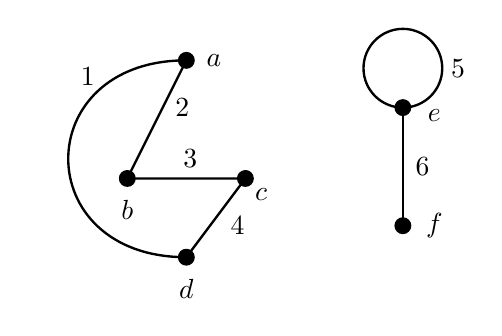
\begin{tikzpicture}
	% 'PacMan'
	\draw[fill=black] (0.75,1.5) circle (0.1); % a pt
	\draw[fill=black] (0,0) circle (0.1); % b pt
	\draw[fill=black] (1.5,0) circle (0.1); % c pt
	\draw[fill=black] (0.75,-1) circle (0.1); % d pt
	
	\node at (1.1,1.5) {$a$};
	\node at (0,-0.4) {$b$};
	\node at (1.7,-0.2) {$c$};
	\node at (0.75,-1.4) {$d$};
	
	\node at (-0.5,1.3) {$1$};
	\node at (0.7,0.9) {$2$};
	\node at (0.8,0.25) {$3$};
	\node at (1.4,-0.6) {$4$};	
	
	% Lollipop
	\draw[line width=0.03cm] (3.5,-0.6) -- (3.5,0.9); % Line Segment
	\draw[line width=0.03cm] (3.5,1.4) circle (0.5); % Circle	
	\draw[fill=black] (3.5,0.9) circle (0.1); % Upper Pt
	\draw[fill=black] (3.5,-0.6) circle (0.1); % Lower Pt
	
	\node at (4.2,1.4) {$5$};	
	\node at (3.9,0.8) {$e$};
	\node at (3.75,0.15) {$6$};
	\node at (3.9,-0.6) {$f$};	
	
	\draw[line width=0.03cm] (0.75,1.5) to[bend right=90, distance=2cm] (0.75,-1); % Left Arc		
	\draw[line width=0.03cm] (0.75,-1) -- (1.5,0) -- (0,0) -- (0.75,1.5); % 'Edges'
	\end{tikzpicture}
	\]

\begin{enumerate}[(a)]
\item What is adjacent to $a$?
\item What is adjacent to 3?
\item Are there parallel edges? Explain.
\item Is the graph connected? Explain.
\item Is the graph simple? Explain. 
\end{enumerate} \pspace

\sol 
\begin{enumerate}[(a)]
\item The vertices $b$ and $d$ are adjacent to $a$. \pspace

\item The edges $2$ and $4$ are adjacent to $3$. \pspace

\item There are no parallel edges because there are no two edges that share \textit{both} endpoints. \pspace

\item The graph is not connected. For instance, there is no walk (sequence of edges) to take one from $a$ to $e$. \pspace

\item The graph is not simple because there is a loop at $e$---namely edge $5$. 
\end{enumerate}



% Question 7
\newpage
\question[10]  Let $G$ be the graph given below:
	\[
	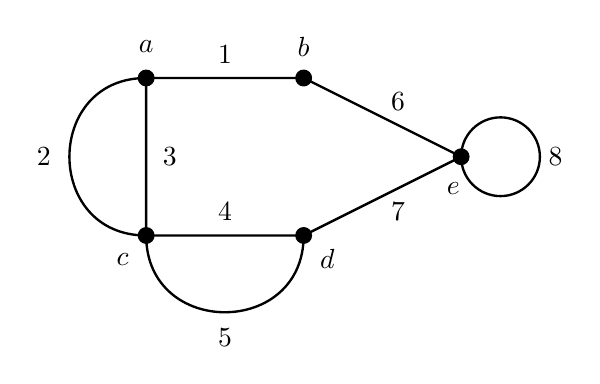
\begin{tikzpicture}
	\draw[line width=0.03cm] (4,1) -- (2,0) -- (0,0) -- (0,2) -- (2,2) -- (4,1);
	\draw[line width=0.03cm] (0,0) to[bend left=90, distance=1.3cm] (0,2);
	\draw[line width=0.03cm] (0,0) to[bend right=90, distance=1.3cm] (2,0);
	\draw[line width=0.03cm] (4.5,1) circle (0.5);
	
	\draw[fill=black] (0,0) circle (0.1);
	\draw[fill=black] (0,2) circle (0.1);
	\draw[fill=black] (2,2) circle (0.1);
	\draw[fill=black] (2,0) circle (0.1);
	\draw[fill=black] (4,1) circle (0.1);
	
	\node at (1,2.3) {$1$};
	\node at (-1.3,1) {$2$};
	\node at (0.3,1) {$3$};
	\node at (1,0.3) {$4$};
	\node at (1,-1.3) {$5$};
	\node at (3.2,1.7) {$6$};
	\node at (3.2,0.3) {$7$};
	\node at (5.2,1) {$8$};
	
	\node at (0,2.4) {$a$};
	\node at (2,2.4) {$b$};
	\node at (-0.3,-0.3) {$c$};
	\node at (2.3,-0.3) {$d$};
	\node at (3.9,0.6) {$e$};
	\end{tikzpicture}
	\]

\begin{enumerate}[(a)]
\item Find the degree of the vertex $c$.
\item Find the degree of the vertex $e$. 
\item Find the degree of the graph. 
\item Give an example of a trail from $a$ to $c$ that is not a path. 
\end{enumerate} \pspace

\sol 
\begin{enumerate}[(a)]
\item $\deg(c)= 4$ \pspace

\item $\deg(e)= 4$ \pspace

\item $\deg G= 2 \cdot \# \text{ edges}= 2 \cdot 8=16$ \pspace

\item Any path that repeats a vertex but not an edge will work as an example. For instance, $a257613c$.
\end{enumerate}



% Question 8
\newpage
\question[10]  Consider the graph below:
	\[
	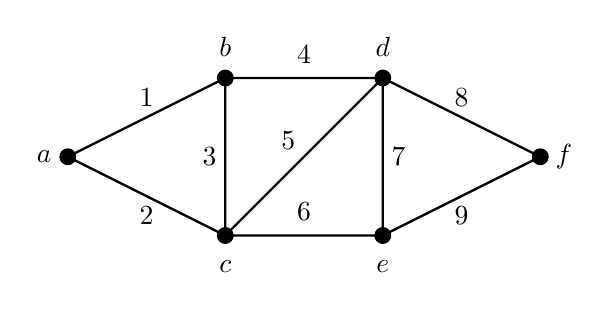
\begin{tikzpicture}
	\draw[line width=0.03cm] (0,2) -- (-2,1) -- (0,0);
	\draw[line width=0.03cm] (2,2) -- (0,2) -- (0,0) -- (2,0) -- (4,1) -- (2,2) -- (2,0);
	\draw[line width=0.03cm] (0,0) -- (2,2);
	
	\draw[fill=black] (-2,1) circle (0.1);
	\draw[fill=black] (0,0) circle (0.1);
	\draw[fill=black] (0,2) circle (0.1);
	\draw[fill=black] (2,0) circle (0.1);
	\draw[fill=black] (2,2) circle (0.1);
	\draw[fill=black] (4,1) circle (0.1);
	
	\node at (-2.3,1) {$a$};
	\node at (0,2.4) {$b$};
	\node at (0,-0.4) {$c$};
	\node at (2,2.4) {$d$};
	\node at (2,-0.4) {$e$};
	\node at (4.3,1) {$f$};
	
	\node at (-1,1.75) {$1$};
	\node at (-1,0.25) {$2$};
	\node at (-0.2,1) {$3$};
	\node at (1,2.3) {$4$};
	\node at (0.8,1.2) {$5$};
	\node at (1,0.3) {$6$};
	\node at (2.2,1) {$7$};
	\node at (3,1.75) {$8$};
	\node at (3,0.25) {$9$};
	\end{tikzpicture}
	\]

\begin{enumerate}[(a)]
\item Explain why the graph does not have an Euler circuit. 
\item Explain why the graph has an Euler trail. 
\item Find an Euler trial for this graph. 
\end{enumerate} \pspace

\sol 
\begin{enumerate}[(a)]
\item A connected graph has an Euler circuit if and only if every vertex has positive even degree. The graph is connected. Vertex $b$ has degree 3, which is odd. So not all vertices have positive even degree. Therefore, the graph does not have an Euler circuit. \pspace

\item A connected graph has an Euler trail if and only if there are exactly vertices with odd degree. Observe that every vertex in the graph has even degree except for vertex $b$ (which has degree 3) and vertex $c$ (which has degree 3). \pspace

\item A possible Euler trail is $b123456789c$.
\end{enumerate}



% Question 9
\newpage
\question[10] Consider the graph below:
	\[
	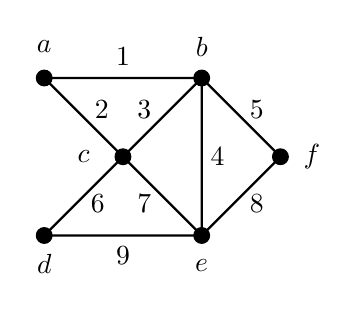
\begin{tikzpicture}
	\draw[line width=0.03cm] (2,2) -- (3,1) -- (2,0) -- (2,2) -- (0,2) -- (1,1) -- (0,0) -- (2,0) -- (1,1) -- (2,2);
	
	\draw[fill=black] (0,0) circle (0.1);
	\draw[fill=black] (2,0) circle (0.1);
	\draw[fill=black] (0,2) circle (0.1);
	\draw[fill=black] (2,2) circle (0.1);
	\draw[fill=black] (1,1) circle (0.1);
	\draw[fill=black] (3,1) circle (0.1);
	
	\node at (0,2.4) {$a$};
	\node at (2,2.4) {$b$};
	\node at (0.5,1) {$c$};
	\node at (0,-0.36) {$d$};
	\node at (2,-0.38) {$e$};
	\node at (3.4,1) {$f$};
	
	\node at (1,2.27) {$1$};
	\node at (0.73,1.6) {$2$};
	\node at (1.27,1.6) {$3$};
	\node at (2.2,1) {$4$};
	\node at (2.7,1.6) {$5$};
	\node at (0.68,0.4) {$6$};
	\node at (1.27,0.4) {$7$};
	\node at (2.7,0.4) {$8$};
	\node at (1,-0.25) {$9$};
	\end{tikzpicture}
	\]

\begin{enumerate}[(a)]
\item Find an Euler circuit for this graph. 
\item Find a Hamiltonian circuit for this graph. 
\end{enumerate} \pspace

\sol 
\begin{enumerate}[(a)]
\item There are many possible Euler circuits for this graph. For instance, the circuit $a136945872a$. \pspace

\item There are many possible Hamiltonian circuits for this graph. For instance, the circuit $a269851a$. 
\end{enumerate}



% Question 10 
\newpage
\question[10] Let $G$ be the graph below:
	\[
	\begin{tikzpicture}
	\begin{scope}[very thick,decoration={
	markings,
	mark=at position 0.5 with {\arrow{>}}
				}
	] 
	\draw[line width=0.03cm,postaction={decorate}] (0,0) -- (2.5,0);
	\draw[line width=0.03cm,postaction={decorate}] (0,0) -- (1.25,2);
	\draw[line width=0.03cm,postaction={decorate}] (1.25,2) -- (2.5,0);
	\draw[line width=0.03cm,postaction={decorate}] (0,0) to[out= -30,in= -150] (2.5,0);
	\draw[line width=0.03cm,postaction={decorate}] (0,0) to[out= 30,in= 150] (2.5,0);
	\draw[line width=0.03cm,postaction={decorate}] (1.25,2) to[out= -30,in= 90] (2.5,0);
	\draw[line width=0.03cm,postaction={decorate},domain= 420:60] plot ({-0.33+0.433*cos(\x)}, {-0.33+0.433*sin(\x)});
	\draw[line width=0.03cm,postaction={decorate},domain= 120:480] plot ({2.83+0.433*cos(\x)}, {-0.33+0.433*sin(\x)});

	\draw[fill=black] (0,0) circle (0.1);
	\draw[fill=black] (2.5,0) circle (0.1);
	\draw[fill=black] (1.25,2) circle (0.1);
	
	\node at (-0.15,0.35) {$1$};
	\node at (1.25,2.4) {$2$};
	\node at (2.7,0.35) {$3$};
	\end{scope}
	\end{tikzpicture}
	\]

\begin{enumerate}[(a)]
\item Find the adjacency matrix for $G$.
\item Find the number of walks from 1 to 3 of length 2. 
\end{enumerate} \pspace

\sol 
\begin{enumerate}[(a)]
\item The adjacency matrix is\dots
	\[
	\begin{pmatrix}
	1 & 1 & 3 \\
	0 & 0 & 2 \\
	0 & 0 & 1
	\end{pmatrix}
	\] \pspace

\item 
	\[
	\begin{aligned}
	A^2&= AA \\[0.3cm]
	&= \begin{pmatrix}
	1 & 1 & 3 \\
	0 & 0 & 2 \\
	0 & 0 & 1
	\end{pmatrix}
	\begin{pmatrix}
	1 & 1 & 3 \\
	0 & 0 & 2 \\
	0 & 0 & 1
	\end{pmatrix} \\[0.3cm]
	&= \begin{pmatrix}
	1(1) + 1(0) + 3(0) & 1(1) + 1(0) + 3(0) & 1(3) + 1(2) + 3(1) \\
	0(1) + 0(0) + 2(0) & 0(1) + 0(0) + 2(0) & 0(3) + 0(2) + 2(1)  \\
	0(1) + 0(0) + 1(0) & 0(1) + 0(0) + 1(0) & 0(3) + 0(2) + 1(1) 
	\end{pmatrix} \\[0.3cm]
	&= \begin{pmatrix}
	1 + 0 + 0 & 1 + 0 + 0 & 3 + 2 + 3 \\
	0 + 0 + 0 & 0 + 0 + 0 & 0 + 0 + 2 \\
	0 + 0 + 0 & 0 + 0 + 0 & 0 + 0 + 1 
	\end{pmatrix} \\[0.3cm]
	&= \begin{pmatrix}
	1 & 1 & 8 \\
	0 & 0 & 2 \\
	0 & 0 & 1
	\end{pmatrix}
	\end{aligned}
	\]
Because $a_{13}= 8$, there are 8 walks of length 2 from 1 to 3. 
\end{enumerate}


\end{questions}
\end{document}